


\chapter[基于输入图片多尺寸放大的卷积神经网络显著图解释方法]{\texorpdfstring{基于输入图片多尺寸放大的卷积神经网络\\显著图解释方法}{基于输入图片多尺寸放大的卷积神经网络显著图解释方法}}\label{MSGCAM}
\thispagestyle{others}
\pagestyle{others}
\xiaosi

\section{引言}
在第\ref{relatedWork}章中介绍了当前几种著名的显著图生成方法,这些方法有基于卷积神经网络的也有基于Transformer架构的,其中几种著名的方法都是应用于卷积神经网络的基于类激活映射的方法,例如Grad-CAM、Grad-CAM++、Score-CAM。因此本章的研究工作就是在这些既有方法的基础上提出了一种基于输入图片多尺寸放大的卷积神经网络显著图解释方法。本章的内容安排如下:首先在\ref{3:problem}节中指出了当前大多数基于类激活映射的显著图解释方法普遍存在的缺点并结合例子分析其原因,然后提出了本章方法的研究思路和解决路径。接着,在\ref{3:method}节中结合算法流程图和算法描述详细介绍了本章的基于输入图片多尺寸放大的卷积神经网络显著图解释方法。随后,在\ref{3:test}中介绍了实验相关的配置和数据集信息,然后进行了直观对比实验验证本章方法显著图的视觉效果,还从定量分析的角度设计了插入和删除实验,定点游戏实验进一步验证了本章方法相比对比方法的有效性和优点。最后在\ref{3:finish}节中总结了本章的工作内容。

\section{问题描述和研究思路}\label{3:problem}
当前大多数基于类激活映射的显著图解释方法诸如CAM、Grad-CAM、Grad-CAM++、XGrad-CAM、Score-CAM等都存在一个共有问题,即最终生成的显著图的分辨率较低,这导致其只能在显著图中呈现一个模糊的解释效果,无法聚焦更加精细的特征。究其原因是这些基于类激活映射的方法一般提取的都是卷积神经网络的最后一层卷积层的输出作为特征图的来源,因该层包含较为丰富的类别特征信息,之后通过各种加权方法组合这些特征图来得到最终的显著图。因为卷积神经网络的结构特性,其最后一层卷积层的会输出多个通道的低分辨率特征图,因此无论如何组合这些特征图,最终得到的也只是一张分辨率和最后一层的卷积层输出的单一通道的特征图相当的初级显著图。当然一般情况下为了得到显著图和原始输入图片的特征对应关系,都会将这张原始输入图片进行分辨率层面的放大,使用的一般也是双线性插值算法,但这并不意味着原始显著图的有效信息的增多。

这里以VGG19这个基于卷积神经网络的图片分类模型举例,若输入图片的尺寸是3$\times$224$\times$224,其中3表示RGB颜色通道,224$\times$224表示图片分辨率,那么该模型最后一层卷积层的输出的特征图尺寸是512$\times$14$\times$14,其中数字512是通道数量,14$\times$14是特征图的分辨率。若使用双线性插值函数$\phi(s,H,W)$将原始显著图分辨率提升到224$\times$224,那么意味着插入了额外99.9\%的信息,而最终的显著图中的这些额外的像素信息并不能反映图片分类模型对原始输入图片的对应像素的感兴趣程度。即便有部分文献\textsuperscript{\cite{adebayo2018sanity,selvaraju2017grad}}试图改进这种插值函数,但是它们仍然引入了外部不相关的信息。

因此为了解决上述的问题,本章从特征图的提取这一关键点着手。考虑到若使用原始输入图片,那么卷积神经网络最后一层卷积层输出的单一特征图分辨率较低且包含的特征信息有限,因此本章提出基于输入图片多尺寸放大的卷积神经网络显著图解释方法,其核心就是将输入图片进行逐级多尺寸的双线性插值放大,例如将输入图片放大至334$\times$334、434$\times$434、534$\times$534等分辨率,这时能得到一组分辨率不同的输入图片,接着将这组输入图片分别送入基于卷积神经网络的图像分类模型中,再从其最后一层卷积层中分别提取特征图和梯度矩阵数据,基于卷积神经网络的采样特性,可以得到不同分辨率的特征图,更高分辨率的输入图片即对应更高分辨率的特征图,也即拥有更丰富的特征信息。因此若将这些特征图的信息进行融合即能得到分辨率更高的掩膜,再用这些更高分辨率的掩膜对原始输入图片进行扰动,即可得到相应的掩膜权重,用权重和高分辨率掩膜进行融合即能得到包含更多特征信息并且分辨率更高的显著图。


\section{基于输入图片多尺寸放大的卷积神经网络显著图解释方法}\label{3:method}
本章提出基于基于输入图片多尺寸放大的卷积神经网络显著图解释方法来解决目前可视化算法结果分辨率低、无法给出更详细目标特征的问题。为了方便本章后文的描述,本章对该方法的简称是MSG-CAM(Multi-Scale inputs of Group-
CAM)。MSG-CAM的算法流程描述参见算法\ref{alg:1},算法流程图参见图\ref{fig:msg_pipeline}。

\begin{figure}[!ht]
	\centering 
	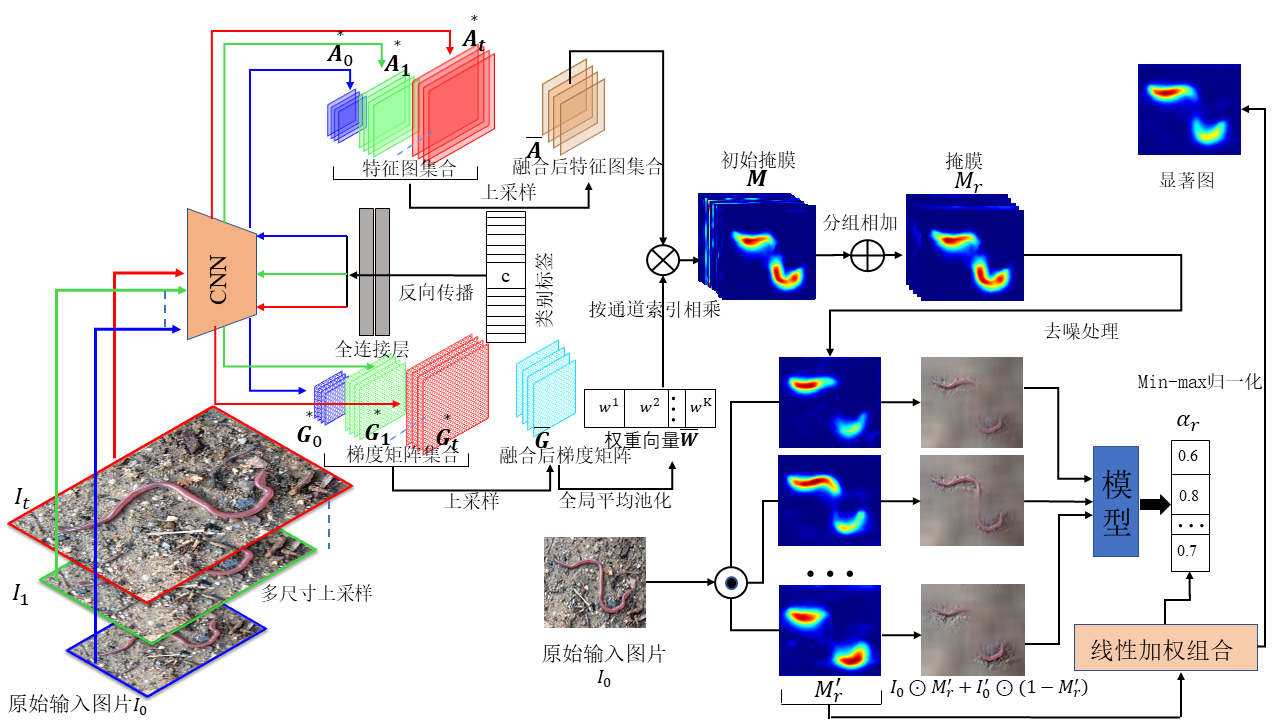
\includegraphics[width=15cm]{fig/ch3/msg_pipeline.png}
	\bicaption[\xiaosi MSG-CAM算法流程示意图]{\wuhao MSG-CAM算法流程示意图}{\wuhao Pipeline of MSG-CAM}
	\label{fig:msg_pipeline}
\end{figure}


\subsection{生成高分辨率掩膜}
令原始输入图片为$I_0 \in \mathbb{R}^{3\times H_0 \times W_0}$,其中3表示RGB颜色通道数量,$H_0$和$W_0$分别原始输入图片的长和宽的像素个数,即原始输入图片的分辨率可以表示为$\zeta_0=(H_0,W_0)$。此外,本章用$\mathcal{F}$表示一个预训练好的基于卷积神经网络的图像分类模型,那么$\mathcal{F}_c(I_0)$则表示在输入图片为$I_0$的情况下,图像分类模型$\mathcal{F}$对于类别$c$的输出分数,值得注意的是,该分数是未经归一化指数函数(softmax函数)之前的分数。将原始输入图片送入图像分类模型$\mathcal{F}$,并从其最后一层卷积层$l$当中提取所有通道的特征图集合,该特征图集合表示为$\overset{*}{\boldsymbol{A}_0}$。通过获得的类别$c$的输出分数$\mathcal{F}_c(I_0)$,对该分数反向传播至最后一层卷积层,则可以获得对应该层特征图关于类别$c$的梯度矩阵$\overset{*}{\boldsymbol{G}_0}$,计算公式如下:
\begin{equation}
\overset{*}{\boldsymbol{G}_0}=\frac{\partial \mathcal{F}_c(I_0)}{\partial \overset{*}{\boldsymbol{A}_0}}
\label{eq:g0}
\end{equation}
\ref{eq:g0}公式中,梯度矩阵集合$\overset{*}{\boldsymbol{G}_0}$一共有$K$个通道,通道数量和特征图集合$\overset{*}{\boldsymbol{A}_0}$一致,并且每个通道的梯度矩阵和特征图一一对应。 

接着将原始输入图片$I_0$经由双线性插值函数$\varphi(I_0,\zeta_t)$上采样至图片$I_t$,$t$表示第$t$次上采样结果,经由上采样后的$I_t$的分辨率可表示为$\zeta_t$,$\zeta_t$是由于原始输入图片的分辨率$\zeta_0$逐步递增得来的。为了控制计算的时间成本,考虑将$\zeta_{max}=(H_{max},W_{max})$作为上采样分辨率的上限,同时设$N$为最大迭代次数即上采样次数,那么第$t$次上采样得到的图片分辨率可由以下公式计算得出:
\begin{equation}
	\zeta_t=\zeta_0 +\lfloor\frac{\zeta_{max}}{N}\rfloor(t-1)
\end{equation}
在上述迭代过程当中,每次上采样获得的输入图片$I_t$的分辨率都不同,则将其输入到图像分类模型当中$\mathcal{F}$从最后一层卷积层提取的特征图集合$\overset{*}{\boldsymbol{A}_t}$的分辨率也不同,而且随着输入图片分辨率的提高,$\overset{*}{\boldsymbol{A}_t}$的分辨率也会相应提高,相对应的$\overset{*}{\boldsymbol{A}_t}$也能包含更多和类别$c$相关的细节特征信息。因此若将这些不同的分辨率的特征图集合进行融合则能够得到更多的特征信息。融合的方法可由以下的公式进行表示:
\begin{equation}
	\overline{\bm{A}}=\frac{1}{t_{max}}\sum_{t=0}^{t_{max}}\varphi(\overset{*}{\boldsymbol{A}_t},\zeta_0)
	\label{eq:Afuse}
\end{equation}
公式\ref{eq:Afuse}中,$t_{max}$表示最大的有效迭代次数,此处的“有效”指的是只有当图像分类模型的输出结果中概率分数最大的类别是$c$时才采用这次迭代的特征图集合$\overset{*}{\boldsymbol{A}_t}$,其他情况下均舍弃,因此不难得出$t_{max} \leq N$。同时$\varphi(\overset{*}{\boldsymbol{A}_t},\zeta_0)$表示将特征图集合$\overset{*}{\boldsymbol{A}_t}$中的每一个通道上的特征图均上采样至原始输入图片的分辨率$\zeta_0$,这样做的目的是方便将不同分辨率的特征图集合进行融合,也方便后续对原始输入图片进行扰动。

在每次迭代过程中,都会计算并提取保存图像分类模型关于类别c的输出分数$\mathcal{F}_c(I_t)$对于卷积层$l$的特征图集合$\overset{*}{\boldsymbol{A}_t}$的反向传播梯度$\overset{*}{\boldsymbol{G}_t}$,和特征图集合一样,将不同迭代过程中保存的梯度矩阵集合$\overset{*}{\boldsymbol{G}_t}$也进行融合,可以得到与$\overline{\bm{A}}$分辨率尺寸一致梯度矩阵集合,融合的公式如下所示:
\begin{equation}
	\overline{\bm{G}}=\frac{1}{t_{max}}\sum_{t=0}^{t_{max}}\varphi(\overset{*}{\boldsymbol{G}_t},\zeta_0)
	\label{eq:Gfuse}
\end{equation}
同样,公式\ref{eq:Gfuse}中,同时$\varphi(\overset{*}{\boldsymbol{G}_t},\zeta_0)$表示将梯度矩阵集合$\overset{*}{\boldsymbol{G}_t}$中的每一个通道上的梯度矩阵均上采样至原始输入图片的分辨率$\zeta_0$。由于融合后的特征图集合中不仅包含类别$c$特征信息,也包含其他类别的特征信息,因此为了将类别$c$的特征信息进行凸显,其他类别的特征信息进行削弱,本方法将利用融合后的梯度矩阵$\overline{\bm{G}}$,它在一定程度上反映了特征图上不同像素对类别分数$\mathcal{F}_c(I_0)$的敏感程度,或者说是重要程度\textsuperscript{\cite{selvaraju2017grad}3}。仿照Grad-CAM\textsuperscript{\cite{selvaraju2017grad}4}中的方法,将$\overline{\bm{G}}$中每张梯度矩阵进行全局平均池化,在每个通道上得到一个权重值,每个通道下的权重值都和$\overline{\bm{A}}$中的每个通道下的特征图一一对应,所有通道下权重值的集合的计算公式如下:
\begin{equation}
	\overline{\bm{W}}=\frac{1}{H_0\times W_0}\sum_{i=1}^{H_0}\sum_{j=1}^{W_0}\overline{\bm{G}}
	\label{eq:Wfuse}
\end{equation}
额外说明的是,融合后的特征图集合$\overline{\bm{A}}$的尺寸是$[1\times K \times H_0\times W_0]$,它对应的权重集合$\overline{\bm{W}}$的尺寸是$[1\times K \times 1\times 1]$,其中$K$就是第$l$层卷积层输出的特征图通道数量。

本小节的最后,初始掩膜集合$\boldsymbol{M}$可以通过以下公式计算得出:
\begin{equation}
	\boldsymbol{M}=	\overline{\bm{A}}\cdot\overline{\bm{W}}
\end{equation}
其中,运算符$\cdot$表示$\overline{\bm{A}}$中的每个通道下的特征图中的每个像素值都和$\overline{\boldsymbol{W}}$中对应每个权值相乘。

\subsection{掩膜优化}
$\boldsymbol{M}$是经由输入图片多尺寸上采样放大后从卷积层中提取的特征图和梯度矩阵结合而得到的,相比单一原始输入图片得到掩膜(比如Score-CAM\textsuperscript{\cite{wang2020score}4-5}),$\boldsymbol{M}$包含更丰富的类别特征信息,但是目前得到$\boldsymbol{M}$仍然不能直接当作掩膜来扰动输入图片,它还有两个明显的缺点。第一点是$\boldsymbol{M}$的尺寸是$[1\times K \times H_0\times W_0]$,其中$K$是卷积层$l$输出的特征图的通道数量,一般取最后一层卷积层作为$l$,因此$K$的值将会是数百至上千,显然这样掩膜的数量太多了,若像Score-CAM\textsuperscript{\cite{wang2020score}4-5}一样逐个将掩膜去扰动原始输入图片得到权值,那样将会极为耗时。第二个缺点$\boldsymbol{M}$就是使用全局平均池化后的梯度作为特征图的权重,由于ReLU函数的零梯度问题\textsuperscript{\cite{zhang2021novel}},这意味着$\boldsymbol{M}$显然会有噪声。因此,为了使$\boldsymbol{M}$成为合格的掩膜,需要让它变得更加纯净。

对于第一个缺陷,本节的解决办法是将$\boldsymbol{M}$中的$K$张掩膜平分为$B$个组,分类依据是它们的相邻关系,接着将每个组内的所有掩膜相加合并为一个掩膜,这个相加合并过程可由以下的公式计算得出:
\begin{equation}
	M_r=ReLU(\sum_{k=r\times g}^{(r+1)\times g-1}{M^k})
	\label{eq:Mr}
\end{equation}
公式\ref{eq:Mr}中$g$是每个组中的特征图的数量且 $g=K/B$,$r$的取值范围是$\{0,1,2,\dots,B-1\}$,即合并完成后一共有$B$张掩膜,$M_r$是第$r$组中合并完成后的掩膜,$M^k$是$\boldsymbol{M}$中第$k$个通道的特征图。

对于第二个缺陷,本方法设计了一个去噪函数$f(m_{ij},\theta)$,该函数中$m_{ij}$是掩膜$M_r$中第$i$行第$j$列的像素值,$\theta$是一个百分比值。具体的去噪计算结果由以下公式计算得出:
\begin{equation}
	f(m_{ij},\theta)= \begin{cases}
		\ m_{ij}, & \rm if \enspace \it m_{ij}>p(M_r,\theta) ; \\
		\ 0, & \rm otherwise .\\
	\end{cases}
\label{eq:denoise}
\end{equation}
公式\ref{eq:denoise}中$p(M_r,\theta)$表示$M_r$的所有像素值从大到小处于$\theta$百分比的值,比如有100个像素值,每个像素值都是1到100中的一个整数取值且取值唯一,此时$\theta =70$,那么$p(M_r,\theta)=70$。\ref{eq:denoise}公式的作用就是将掩膜$M_r$中百分比前$\theta$大的像素值保留,小于$p(M_r,\theta)$的像素值置为0。经过去噪操作后可以得到更加纯净的掩膜。

到目前为止,还剩下最后一个操作即可得到最终的掩膜。将$M_r$中的所有像素值进行最大最小归一化,使其像素值区间位于$[0,1]$,这样方便将掩膜直接和输入图片相乘进行扰动操作。具体计算公式如下:
\begin{equation}
	M^{\prime}_r=\frac{M_r-min(M_r)}{max(M_r)-min(M_r)}\label{e_minmax}
\end{equation}
最后,掩膜$M^{\prime}_r$有这和原始输入图片$I_0$一致的分辨率且掩膜的像素值和$I_0$中的像素值一一对应。

\subsection{生成显著图}
如果显著性方法确实识别出了对模型预测有重要意义的像素,那么这一点就应该反映在重建图像的模型输出当中\textsuperscript{\cite{kapishnikov2019xrai}}。将$M^{\prime}_r$作为掩膜来扰动原始输入图片$I_0$,其背后的原理是从原始输入图像中保留掩膜中获得的关于类别$c$的特征信息,让图像分类模型来判断保留的这部分信息的重要性,判断依据就是图像分类模型对扰动后的图片关于类别$c$的输出概率分数。但是,如果直接将掩膜和原始输入图像相乘进行扰动,那么扰动后的图像中的被掩盖区域和被凸显的区域之间的边界会过于明显锐利,从而对图像分类神经网络造成对抗效果\textsuperscript{\cite{dabkowski2017real}}。

为了遇到避免上述的问题,高斯模糊函数被引入到了接下来的改进方法中。具体方法是将扰动区域即被掩膜遮盖的区域用高斯模糊后的原始输入图片的对应区域进行替代,这样可以使得凸显的图片区域和被扰动的图片区域之间的边界更加平滑,从而像真实图片,不易让图像分类神经网络产生异常的输出。对于单一掩膜$M^{\prime}_r$,这个扰动模式可以由以下的公式计算得出:
\begin{equation}
	I_r=I_0\odot M^{\prime}_r+I^{\prime}_0\odot (1-M^{\prime}_r)
	\label{eq:Ir}
\end{equation}
公式\ref{eq:Ir}中,$I^{\prime}_0$是将原始输入图片$I_0$高斯模糊后的得到的,$I^{\prime}_0$作为一张基础图片送入图像分类模型$\mathcal{F}$当中,当然得到其关于类别$c$的输出结果$\mathcal{F}_c(I^{\prime}_0)$是一个非常低的值且趋近于0。具体的高斯模糊函数是$guassian\_blur2d(input,kernel\_size,sigma)$,在本章中,参照Group-CAM\textsuperscript{\cite{zhang2021novel}5}的工作,设置高斯模糊的参数$kernel\_size=51$和$sigma=50$。 $1-M^{\prime}_r$表示$M^{\prime}_r$中每个像素值都作为减数被1相减,作用是将掩膜中关于类别$c$的特征信息进行凸显。

参考RISE\textsuperscript{\cite{petsiuk2018rise}5-8}中的方法,每张掩膜$M_r$的权重$\alpha_r$可以由扰动后的$I_r$输入到图像分类模型$\mathcal{F}$中得到。$\mathcal{F}_c(I_r)$则是该权重,其表示模型对显著图区域中类别$c$的特征信息的感兴趣程度。具体计算公式由以下式子给出:
\begin{equation}
	\alpha_r=\mathcal{F}_c(I_r)-\mathcal{F}_c(I^{\prime}_0)
\end{equation}
最终的显著图即将所有$M_r$的权重$\alpha_r$和其本身相乘,并经过ReLU函数后得到,ReLU函数的作用是保留显著图中的正值,即模型关于类别$c$感兴趣的像素区域。具体式子如下表示:
\begin{equation}
	L_{MSG-CAM}=ReLU(\sum_{r}\alpha_r M_r)
\end{equation}
 
\begin{algorithm}[!ht]
 	\caption{MSG-CAM}
 	\label{alg:1}
 	\renewcommand{\algorithmicrequire}{\textbf{输入:}}
 	\renewcommand{\algorithmicensure}{\textbf{输出:}}
 	\begin{algorithmic}[1]
 		\REQUIRE 基于卷积神经网络的图像分类模型 $\mathcal{F} $ ,原始输入图片 $I_0 \in \mathbb{R}^{3\times H_0 \times W_0}$ ,上采样分辨率上限 $\zeta_{max}=(H_{max},W_{max})$ ,卷积层 $l$ ,最大迭代次数 $N$ ,类别 $c$ ,每个分组中掩膜数量$B$, 高斯模糊参数: $kernel\_size,sigma$, 上采样插值函数 $\varphi(.)$
 		\ENSURE 显著图 $L_{MSG-CAM}\in \mathbb{R}^{3\times H_0 \times W_0}$
 		\STATE 初始化 $L_{MSG-CAM} \leftarrow 0$ , $\mathcal{A}_0 \leftarrow 0$ , $\mathcal{G}_0 \leftarrow 0$ , $r \leftarrow 0$ , $t_{max}\leftarrow 0$ , $t_m\leftarrow 0$ , $kernel\_size=51,sigma=50$ ,基准图片 $I^{\prime}_0=guassian\_blur2d(I_0,kernel\_size,sigma)$ , $c=\mathcal{F}(I_0)$
 		\WHILE{$t\leq N$}
 		\STATE $t\leftarrow t+1$
 		\STATE $\zeta_t\leftarrow \zeta_0 +\lfloor\frac{\zeta_{max}}{N}\rfloor(t-1)$
 		\STATE $I_t\leftarrow \varphi(I_0,\zeta_t)$
 		\IF{$\mathcal{F}(I_t) \rightarrow c$}
 		\STATE $t_{max}\leftarrow t_{max}+1$
 		\STATE $\overset{*}{\boldsymbol{A}_t}\leftarrow \mathcal{A}(I_t,l)$
 		\STATE $\overset{*}{\boldsymbol{G}_t}\leftarrow \nabla\mathcal{J}(l,c)$
 		\STATE $\mathcal{A}_t \leftarrow \mathcal{A}_{t-1}+\varphi(\overset{*}{\boldsymbol{A}_t},\zeta_0)$
 		\STATE $\mathcal{G}_t \leftarrow \mathcal{G}_{t-1}+\varphi(\overset{*}{\boldsymbol{G}_t},\zeta_0)$
 		\ENDIF
 		\ENDWHILE
 		\STATE $\overline{\bm{A}}\leftarrow \mathcal{A}_t/t_{max}$
 		\STATE $\overline{\bm{G}}\leftarrow \mathcal{G}_t/t_{max}$
 		\STATE $\overline{\bm{W}}\leftarrow \frac{1}{m\times n}\sum_{i=i}^{m}\sum_{j=1}^{n}\overline{\bm{G}}$
 		\STATE $\boldsymbol{M}=\overline{\bm{A}}\cdot\overline{\bm{W}}$
 		\STATE $K\leftarrow$ $\boldsymbol{M}$的通道数量;
 		\STATE $g\leftarrow$ 每个分组中掩膜数量;
 		\WHILE{$r<B$}
 		\STATE 在组内生成单一的掩膜\\ $M_r=ReLU(\sum_{k=r\times g}^{(r+1)\times g-1}M^k)$
 		\STATE 初始化 $M^{\prime}_r\leftarrow$ 将$M^r$进行去噪操作和归一化
 		\STATE 用掩膜扰动原始输入图片\\$I_r=I_0\odot M^{\prime}_r+I^{\prime}_0\odot (1-M^{\prime}_r)$
 		\STATE 计算每张掩膜的权重\\$\alpha_r=\mathcal{F}_c(I_r)-\mathcal{F}_c(I^{\prime}_0)$
 		\STATE $L_{MSG-CAM}\leftarrow L_{MSG-CAM}+\alpha_r M_r$
 		\STATE $r\leftarrow r+1$
 		\ENDWHILE
 		\RETURN $ReLU(L^c_{MSG-CAM})$
 	\end{algorithmic}
 \end{algorithm}

 
 
\section{实验与分析}\label{3:test}

\subsection{实验硬件配置和软件环境}
下面给出本章实验的硬件配置和实验环境相关信息,具体信息 见表\ref{tab:en}。

\begin{table}
	\renewcommand{\arraystretch}{1.5}
\centering
\bicaption[\xiaosi 实验环境和硬件配置]{\wuhao 实验环境和硬件配置}{\wuhao Experimental environment and hardware configuration}
\label{tab:en}
	\begin{tabular}{p{4cm}p{8cm}} 
\hline
类型                  & \multicolumn{1}{c}{配置信息}      \\ 
\hline
\multirow{3}{*}{硬件} & CPU:10-core Intel$^\circledR$ Xeon$^\circledR$ W-2255 CPU                  \\
& 内存:128GB 64-bit DDR4 3700MHz  \\
& 显卡:NVIDIA RTX A5000 24GB      \\ 
\hline
\multirow{6}{*}{软件} & 操作系统:Ubuntu 20.04 LTS         \\
& Python版本:Python3.8            \\
& 深度学习框架:Pytorch 1.10.1         \\
& 计算架构:CUDA 11.4                \\
& 计算加速库:CUDNN 8.2.0             \\
& AI性能:27.8 TFLOPS              \\
\hline
\end{tabular}
\end{table}


\subsection{数据集及其预处理和实验参数说明}
在本章的实验当中,主要使用了三个数据集,下面是三个数据集的简要介绍:
(1)ILSVRC 2012数据集
ILSVRC 2012(ImageNet Large Scale Visual Recognition Challenge 2012)\textsuperscript{\cite{ILSVRC}}是一个用于视觉对象识别和定位的大规模数据集和竞赛。该数据集包含超过120万张标注图片,涵盖1000个不同类别的物体和场景。ILSVRC 2012竞赛旨在推动计算机视觉领域的发展,参与者需要开发能够识别图像中物体类别的算法,并对物体进行定位。该竞赛对于深度学习和卷积神经网络等技术的发展起到了重要推动作用,成为了评估图像识别算法性能的重要基准。ILSVRC 2012数据集的发布和竞赛对于推动计算机视觉领域的发展产生了深远影响。

(2)PASCAL VOC数据集
PASCAL VOC(Visual Object Classes)\textsuperscript{\cite{pascal}}数据集是一个常用的计算机视觉数据集,用于目标检测、图像分割和场景分类等任务。该数据集最初由牛津大学的计算机视觉研究组创建,包含了20个常见的物体类别,如人、狗、猫、飞机等。数据集中的图像来自于自然场景和网络图像,每个图像都标注了包含的物体类别和位置信息。PASCAL VOC数据集被广泛应用于评估目标检测和图像分割算法的性能,是计算机视觉领域中的重要基准数据集之一。同时,PASCAL VOC数据集也被用于举办国际性的计算机视觉竞赛,吸引了全球的研究者和工程师参与。通过使用PASCAL VOC数据集,研究人员可以开发和评估各种视觉任务的算法,推动计算机视觉技术的发展。

(3)COCO2014数据集
COCO2014数据集(Common Objects in Context)\textsuperscript{\cite{coco}}是一个用于计算机视觉任务的大型数据集,包含超过200,000张图像和相关的注释信息。这些图像涵盖了80个不同类别的物体,并且每张图像都有多个物体的标注,这使得数据集在目标检测、图像分割和物体识别等任务中非常有用。COCO2014数据集的引入为计算机视觉领域的研究和发展提供了重要的资源,成为了许多视觉任务的标准基准。研究人员和开发者可以利用该数据集进行模型训练、算法评估和性能比较,从而推动计算机视觉技术的进步。COCO2014数据集的广泛应用促进了目标检测、图像分割和物体识别等领域的发展,为相关领域的研究和应用提供了有力支持。

在本章当中插入与删除实验中使用的是ILSVRC 2012验证集,包含50000张图片,并且将该验证集中的图片尺寸调整为3$\times$224$\times$224,其中$3$是表示RGB颜色通道数量,像素值进行归一化调整,调整后的像素值范围是[0, 1],最后使用Imagenet数据集的均值[0.229, 0.224, 0.225]和方差[0.485, 0.456, 0.406]对所有图片像素值进行标准化处理。在定点游戏实验中,使用了两个数据集,分别是PASCAL VOC数据集中的测试集,包含4952张图片,和COCO 2014数据集的验证集,包含50000张图片。用于本章实验的图像分类神经网络模型是torchvision提供的预训练模型VGG19\textsuperscript{\cite{simonyan2014very}},它是基于卷积神经网络架构的。如果没有特别说明,本章提出的方法MSG-CAM的默认设置参数是$B=32$,$\theta=70$。所有方法生成的最终显著图默认都上采样至224$\times$224的分辨率。

\begin{figure}[!ht]
	\centering 
	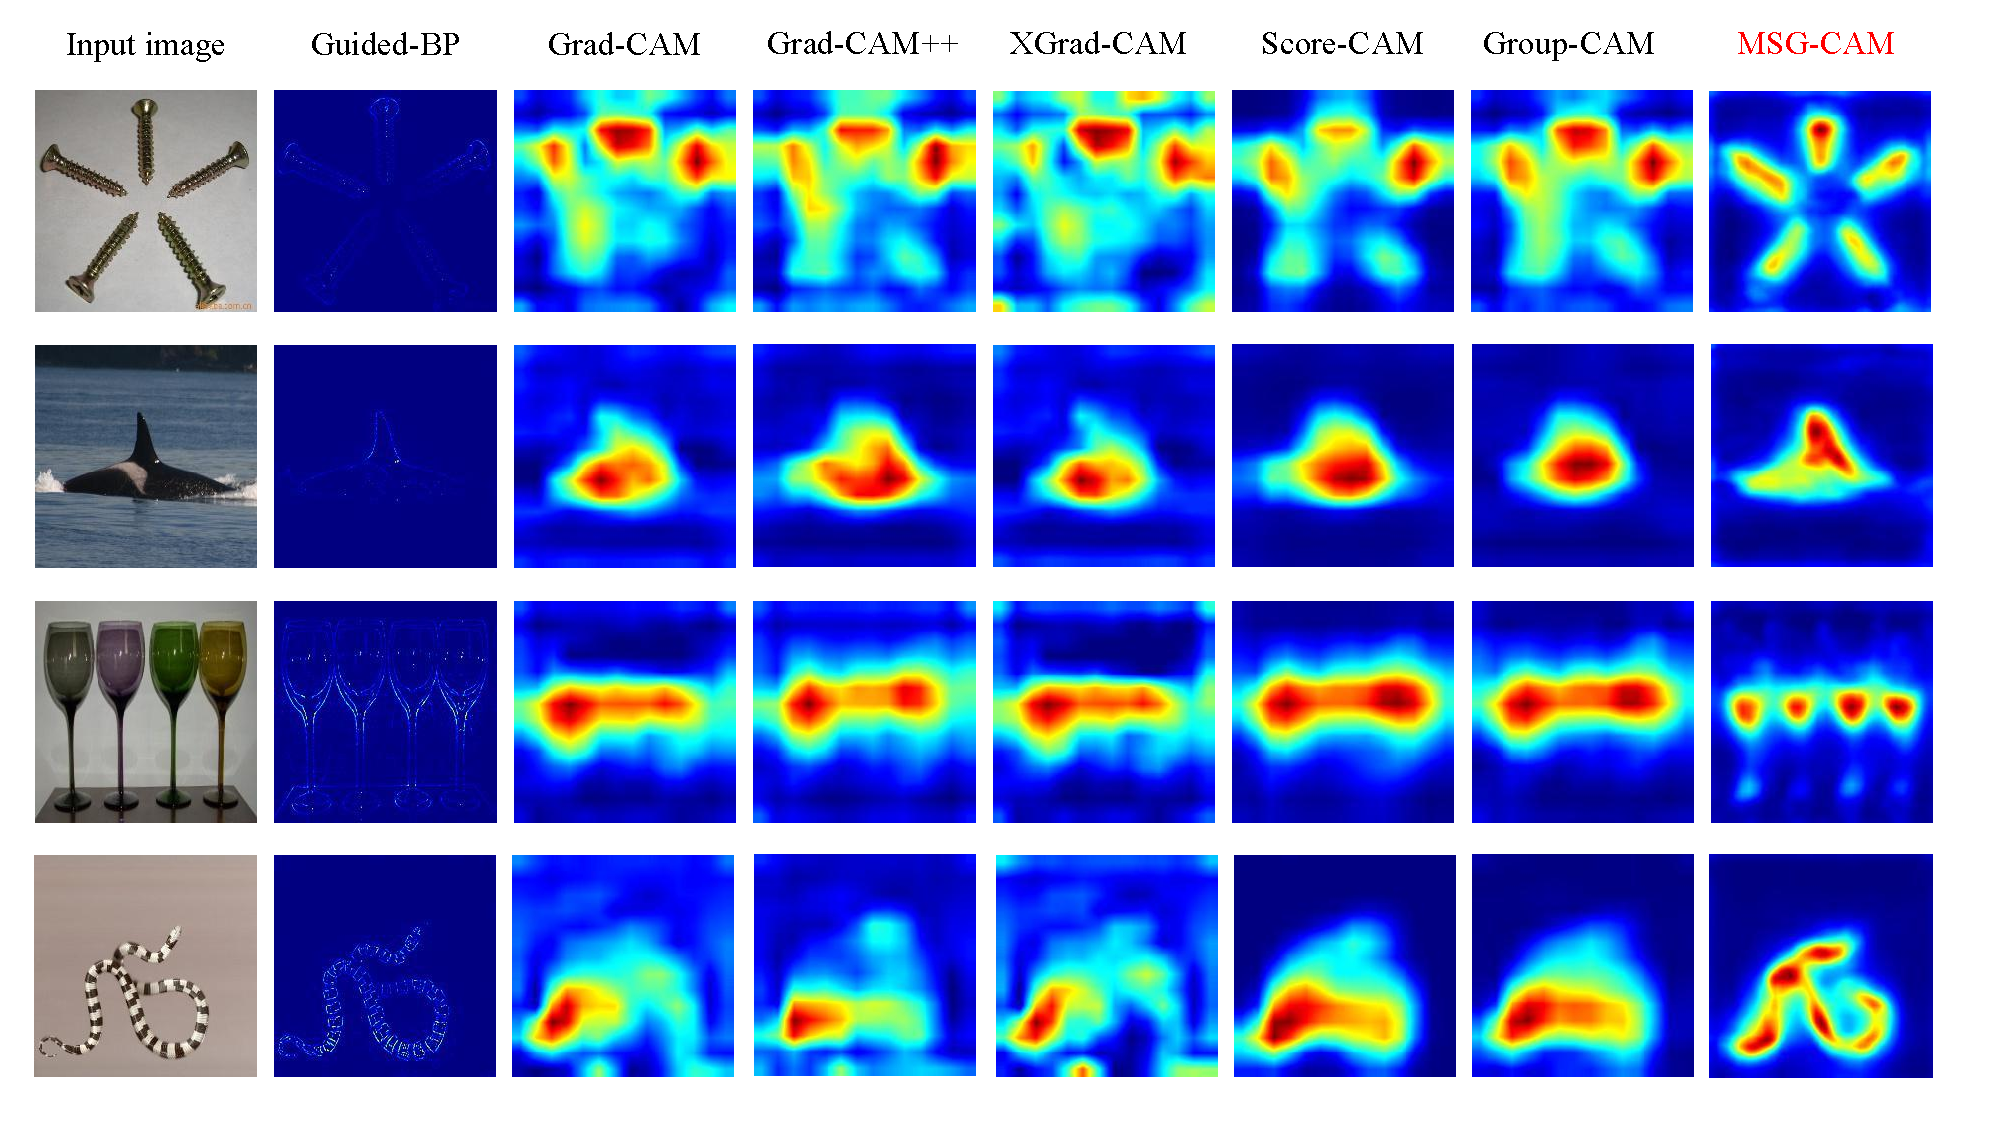
\includegraphics[width=15cm]{fig/ch3/msgContrast.pdf}
	\bicaption[\xiaosi MSG-CAM和其他方法直观对比]{\wuhao MSG-CAM和其他方法直观对比}{\wuhao Visual comparison of MSG-CAM and other methods}
	\label{fig:msgContrast}
\end{figure}

\begin{figure}[!ht]
	\centering 
	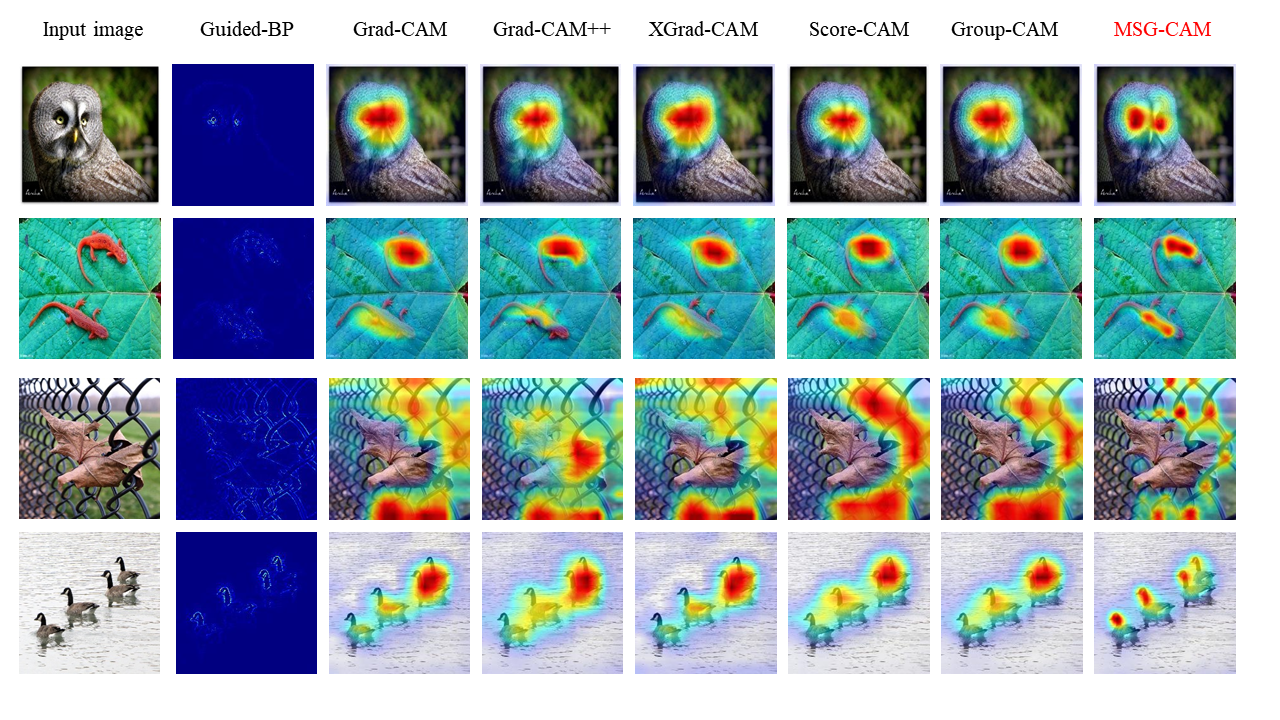
\includegraphics[width=15cm]{fig/ch3/msgContrast2.png}
	\bicaption[\xiaosi MSG-CAM和其他方法直观对比]{\wuhao MSG-CAM和其他方法直观对比}{\wuhao Visual comparison of MSG-CAM and other methods}
	\label{fig:msgContrast2}
\end{figure}
\subsection{直观评估}
直观评估对比是随机从数据集中选取图片,利用显著图生成方法对图片中的目标类别生成显著图,并观察图像分类神经网络对输入图片中哪一部分区域或者哪一部分特征比较感兴趣从而做出了输出类别预测结果。直观评估对比可以明显的比较不同显著图生成方法在相同图片下的显著图结果,可以帮助发现显著图生成算法的不足。

本节随机从ILSVRC 2012数据集的验证集中随机选取了上百张图片进行直观评估对比实验,其中一些图片的显著图的直观对比结果展示在图\ref{fig:msgContrast}和图\ref{fig:msgContrast2}当中。在图\ref{fig:msgContrast}中只展示了输入图片生成的显著图,方便直接对比显著图生成质量。可以在图\ref{fig:msgContrast}明显看出本章提出的MSG-CAM方法生成的显著图具有更高的分辨率,能够更加清晰的给出目标物体特征信息,例如第一行的输入图片类别是“钉子”,只有MSG-CAM能够分别给出五个钉子的轮廓特征信息,第二行的输入图片是“鲸鱼”,只有MSG-CAM给出了图像分类模型判断依据的特征是鱼鳍的轮廓。图\ref{fig:msgContrast2}中第一行输入图片类别是“猫头鹰”,本章提出的MSG-CAM能够明确将猫头鹰的特征锁定在它的两个眼睛上,而其他方法也大多模糊的将特征定位在整个面部。通过直观评估对比,可以较为明显的看出本章提出的MSG-CAM生成的特征图展现出分辨率高,特征呈现更为明确的优势。



\subsection{插入和删除实验}
插入和删除实验首次在RISE\textsuperscript{\cite{petsiuk2018rise}}实验中提出。插入实验背后所反映的原理是按照显著图给出的像素重要程度优先级开始在原图的对应位置逐渐插入重要的像素直至完全插入所有像素,在此过程中记录每次插入操作时模型对指定类别给出的可能性概率分数。插入实验可以衡量显著图对像素重要性的排序是否与模型实际决策时关注的像素重要性排序一致。与之相反的是,删除实验则是按照显著图中给出的像素重要程度优先级逐渐从原输入图片中抹去对应的像素信息。和插入实验一样,删除实验也要求记录每次删除操作后模型对感兴趣类别给出的可能性分数。删除实验可以直观的呈现出缺失重要特征的像素信息后模型对感兴趣类别的置信程度下降情况。

具体而言,对于插入实验,将原输入图片高斯模糊化后作为画布,随后每次迭代过程中,按照显著图给出的像素优先级逐渐向画布中对应的位置中引入原输入图片的像素,每次迭代过程中记录模型对引入像素后的的图片关于指定类别的可能性概率分数。为了更加精确的反映显著图的像素优先级,每次迭代只引入约0.89\%(224$\times$2)的像素。和插入实验相对比,删除实验每次迭代将原输入图片中的像素逐渐替代为画布上的像素,直到输入图片被完全替换为画布为止。删除实验每次迭代仍然是变更约0.89\%的在原图中的像素。

要特别说明的是,引入高斯模糊后的原输入图片作为画布是为了避免引入像素或者删除像素时产生过于锐利的边界,从而更加接近真实图片,避免产生对抗攻击的样本。此外,每次迭代记录的可能性分数都是经过softmax函数进行归一化后的数据。得到插入实验和删除实验每次迭代获得的分数后,使用概率分数随插入或者删除次数的曲线的曲线下面积(Area Under Curve)作为的作为量化指标。为了总体衡量插入实验和删除实验的优劣,增加了总体分数的实验指标。按照上面关于插入实验和删除实验的描述,AUC(插入)越高表明显著图越准确,同理,AUC(删除)越低越好。因此,总体分数计算方式是AUC(总体)减去AUC(删除)。

图\ref{fig:IDCurve}展示了Grad-CAM、Score-CAM、Group-CAM和MSG-CAM为所选的4幅代表性图像生成了显著图以及相应的插入和删除曲线。对于删除曲线,更好的显著图解释方法给出的显著性图应尽可能快地下降,插入曲线与删除曲线正好相反。从图中可以看出本章提出的MSG-CAM在视觉解释效果以及插入删除曲线的表现来看均优于其他三种基于类激活映射的方法。
\begin{figure}[!ht]
	\centering 
	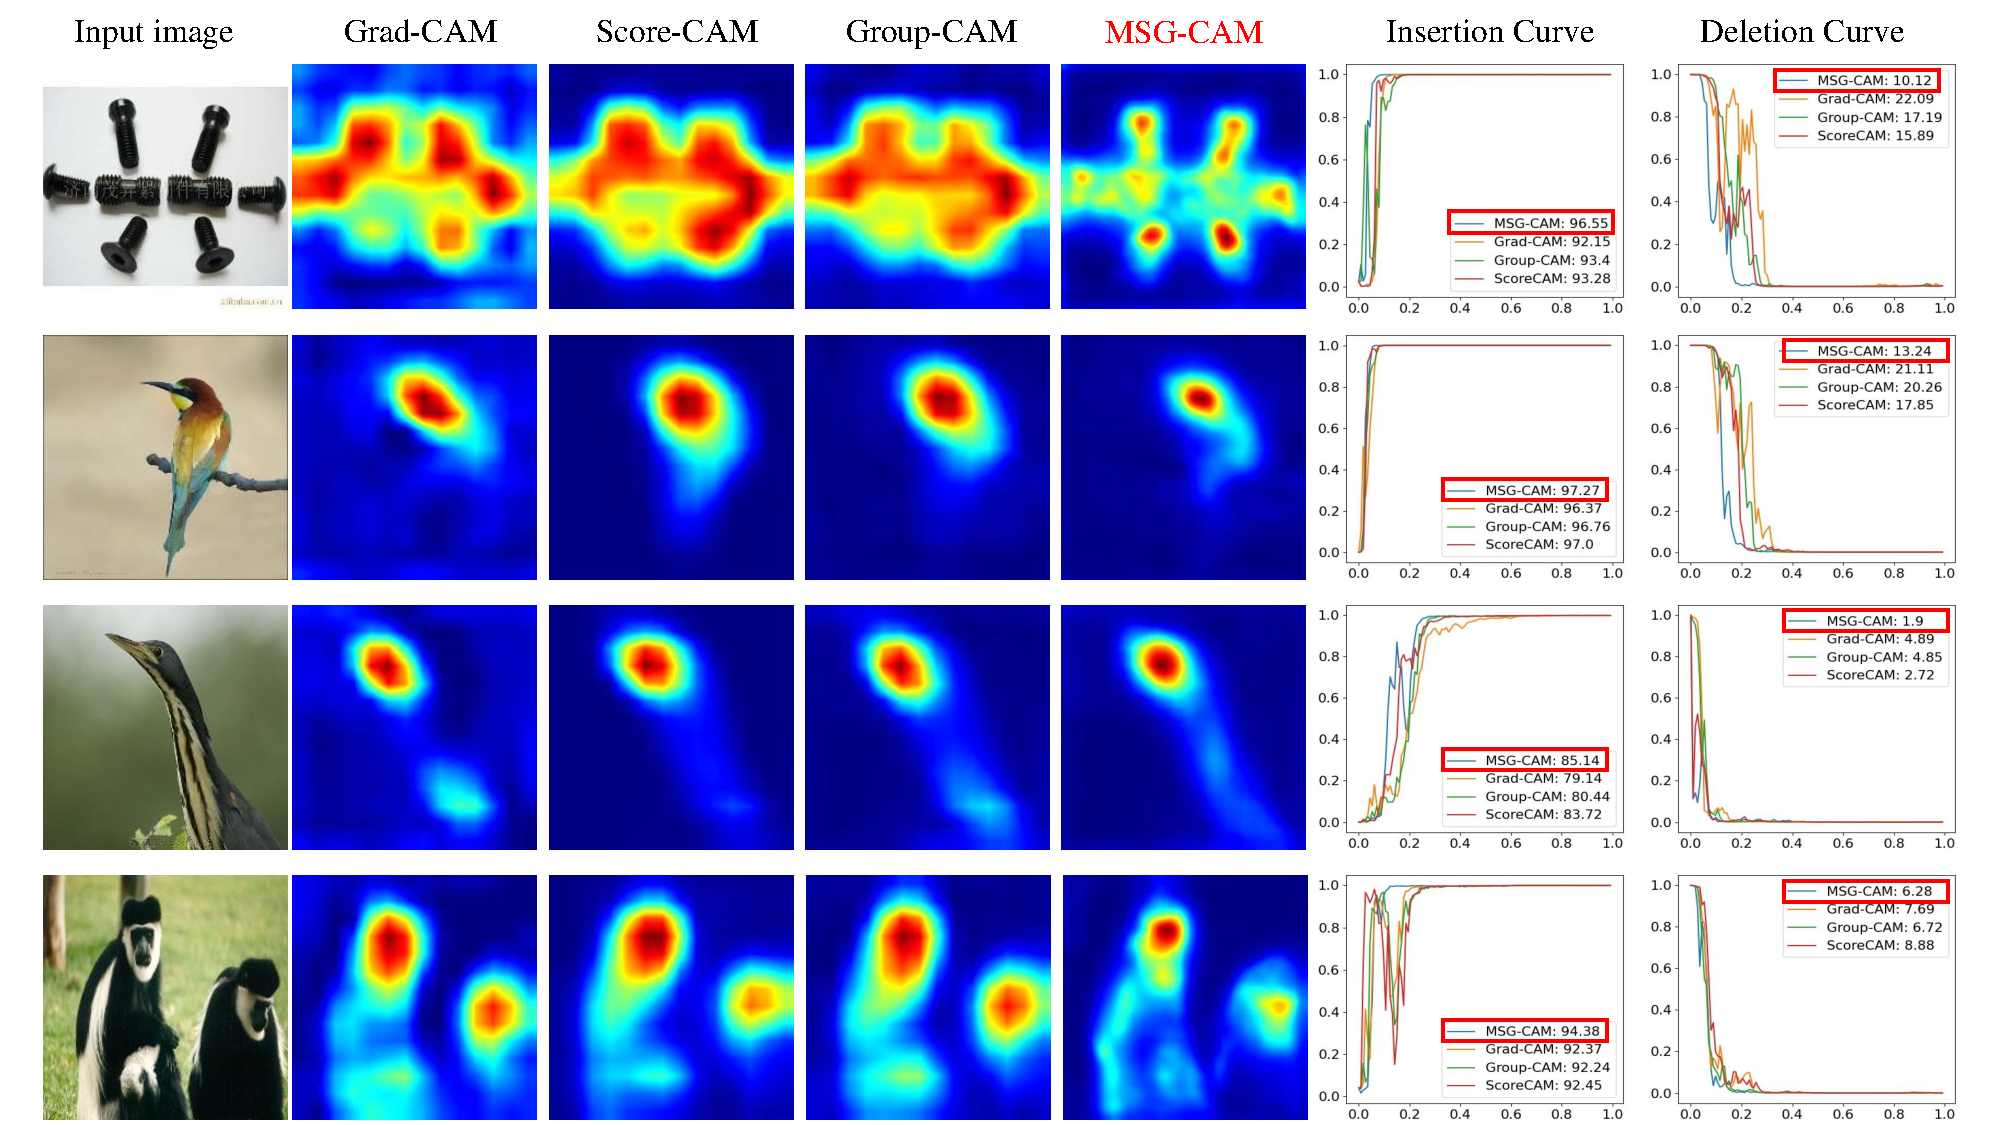
\includegraphics[width=15cm]{fig/ch3/IDCurve.pdf}
	\bicaption[\xiaosi 单张图片在不同方法下的插入删除实验曲线对比]{\wuhao 不同方法下的插入删除实验曲线对比图}{\wuhao Comparison of experimental curves of insertion and deletion under different methods}
	%	\bicaption[\xiaosi MSG-CAM算法流程示意图]{\wuhao MSG-CAM算法流程示意图}{\wuhao Pipeline of MSG-CAM}
	\label{fig:IDCurve}
\end{figure}

\begin{table}[!ht]
	\renewcommand{\arraystretch}{1.5}
	\centering
	\bicaption[\xiaosi 插入和删除实验指标对比]{\wuhao 插入和删除实验指标对比}{\wuhao Comparison of insertion and deletion experiment metrics}
	\wuhao
	\label{auc}
	\begin{tabular}{ccccccc} 
		\toprule[1.5pt]
		AUC & Grad-CAM & Grad-CAM++ & XGrad-CAM & Score-CAM        & CAMERAS       & \textbf{MSG-CAM}  \\ 
		\hline
		插入  & 53.19   & 51.57     & 52.57    & \textbf{55.10}     & 44.10         & 54.52             \\
		删除  & 11.52   & 12.16     & 11.53    & 11.43              & \textbf{8.01} & 9.78              \\
		总体  & 41.67   & 39.41     & 41.04    & 43.67              & 36.09         & \textbf{44.74}    \\
		\bottomrule[1.5pt]
	\end{tabular}
\end{table}
\vspace{-0.3cm}

表\ref{auc}列出了在50000张图像上进行插入和删除的实验结果。虽然MSG-CAM在单项指标上并不突出,但在AUC(总体)这项指标上却是第一名,比第二名的 Score-CAM高出1.07\%。此外,为了探究图像分类神经网络对目标类别的置信程度与三个指标之间的关系。根据每幅图像的分类类别的的最大得分将其分为11组,并统计每组的AUC(插入),AUC(插入)和AUC(总体),统计数据绘制成了图\ref{IDO}。 从图中可以看出,当图像的分类类别的概率分数较低时,各种显著图解释方法之间很难拉开差距。随着图像的分类类别的概率分数的上升,MSG-CAM逐渐显示出优势。在图像的分类类别的概率分数大于等于99.99\%时,即当图像分类神经模型对这组图像中的分类类别有很高的置信度时,MSG-CAM在AUC(总体)有着明显领先。这表明,当图像分类神经网络接近完美的学习到相关类别信息时,MSG-CAM能准确反映这种情况。


\begin{figure*}[!ht]
	\centering
	\bicaption[\xiaosi 分组数据的插入删除实验指标曲线对比图]{\wuhao 分组数据的插入删除实验指标曲线对比图}{\wuhao Insertion and deletion of grouped data experimental metrics curve comparison plot}
	\subfigure[Insertion score divides into segments]{
		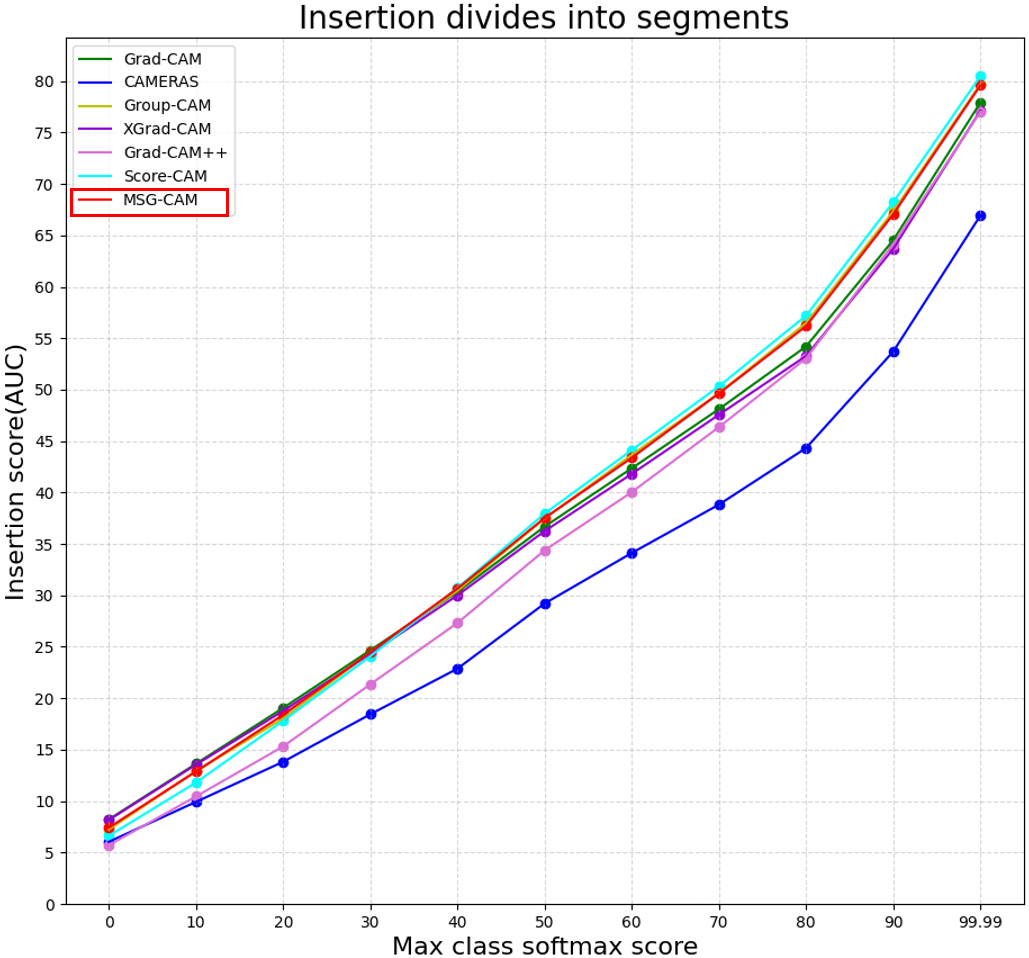
\includegraphics[width=7.2 cm]{fig/ch3/insertion.png}
	}
	\subfigure[deletion score divides into segments]{
		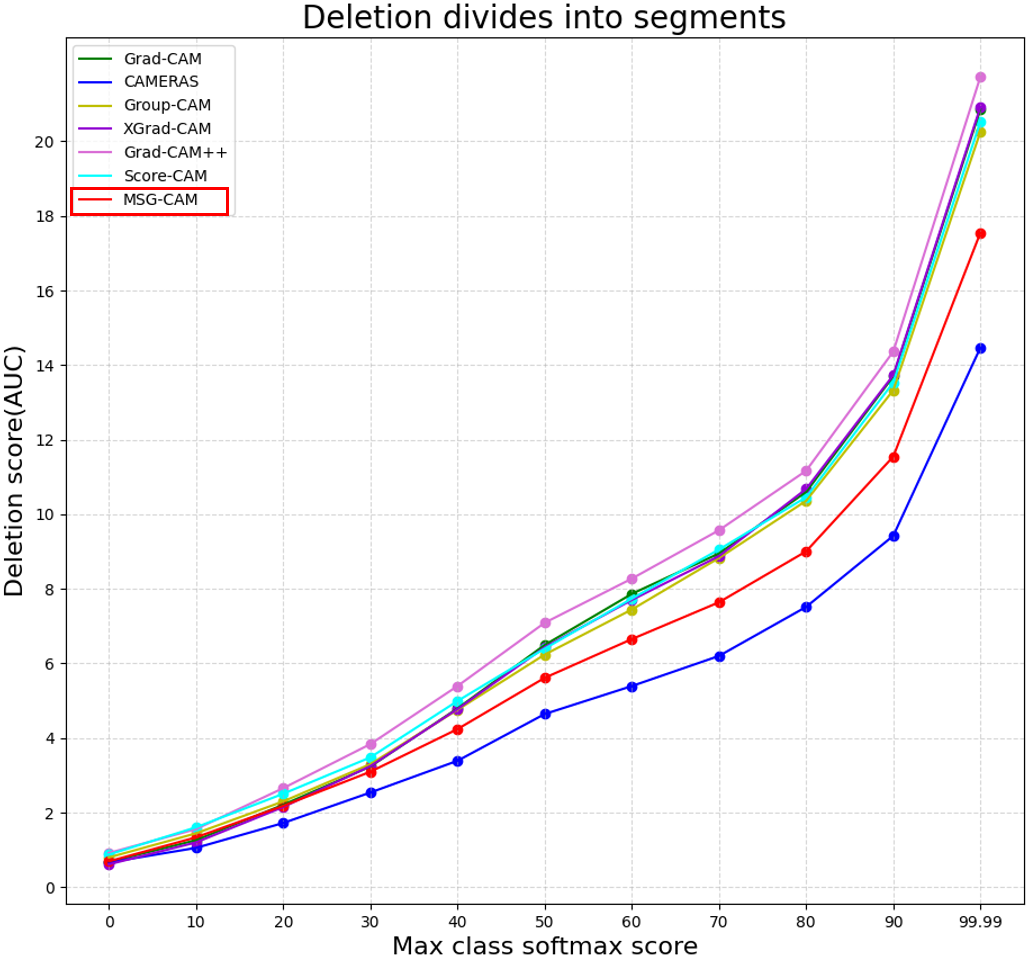
\includegraphics[width=7.2cm]{fig/ch3/deletion.png}
	}
	\subfigure[over-all score divides into segments]{
		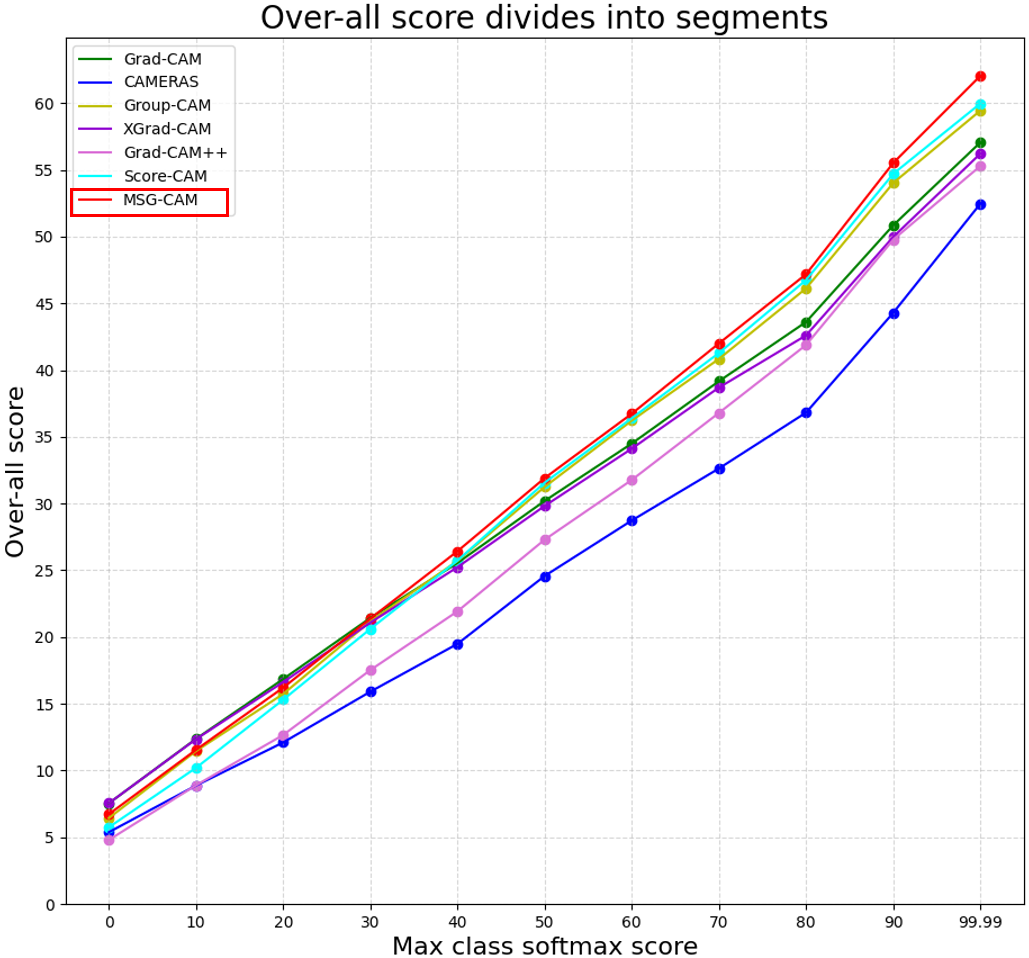
\includegraphics[width=10cm]{fig/ch3/overall.png}
	}
	% \quad
	\label{IDO}
\end{figure*}






\begin{table}
	\renewcommand{\arraystretch}{1.5}
	\centering
	\bicaption[\xiaosi 两个数据集上定点游戏实验平均准确率对比]{\wuhao  两个数据集上定点游戏实验平均准确率对比}{\wuhao Comparison of mean accuracy of pointing game experiments on the two datasets}
	\wuhao

	\begin{tabular}{ccccccc} %需要10列
		\toprule[1.5pt] %添加表格头部粗线
		\multicolumn{2}{c}{\multirow{2}{*}{Method}}& \multicolumn{2}{c}{PASCAL VOC test}&&\multicolumn{2}{c}{COCO 2014 validation}\\
		\multicolumn{2}{c}{}&&Mean Accuracy($\%$)&&Mean Accuracy($\%$)&\\  %有n个&,就表示该行有n+1列
		\hline %绘制一条水平横线
		\multicolumn{2}{c}{Grad-CAM}&   &83.04&    &55.50&    \\   % 占两列,列名为A;后面陆续跟着数字
		\multicolumn{2}{c}{Grad-CAM++}&   &83.21&    &52.91&   \\
		\multicolumn{2}{c}{XGrad-CAM}&   &86.70&    &55.93&   \\
		\multicolumn{2}{c}{Score-CAM}&   &73.92&   &51.20&   \\
		\multicolumn{2}{c}{Group-CAM}&   &82.41&  &54.14&   \\
		\multicolumn{2}{c}{CAMERAS}&   &87.16&    &55.40&   \\
		\multicolumn{2}{c}{\textbf{MSG-CAM}}&   &\textbf{87.24}&   &\textbf{56.62}&   \\
		\bottomrule[1.5pt] %添加表格底部粗线
	\end{tabular}

	\label{point}
\end{table}




\subsection{定点游戏实验}
定点游戏(pointing game)\textsuperscript{\cite{zhang2018top}4-6}实验对于给定显著图解释方法的空间选择性能够给出比较客观的评估结果。所谓空间选择性就是定点游戏要求图像分类神经网络对给定类别在输入图片中指出其所在位置,这对显著图解释方法提出了挑战,方法生成的显著图必须要准确反映给定类别在输入图片的具体位置。定点游戏的具体操作是从针对一个指定类别生成的显著图中找到值最大的那个点并记录它的坐标,如果该坐标位于该类别对象的预先人工标注的边界框内部,则记录一次击中(hit),否则就是没有击中(miss)。定点游戏的量化评价指标即是显著图解释方法在给定数据集上对输入图片中所有类别的击中准确率,具体计算公式如下:
\begin{equation}
	Acc=\frac{\#hits}{\#hits+\#misses}
\label{eq:point}
\end{equation}
式\ref{eq:point}中,$\#hits$表示数据集中所有显著图的最大值点落在标注框中的个数,$\#misses$则表示数据集中所有显著图的最大值点落在标注框外的个数。在只计算最大值空间选择性的定点游戏当中,$\#hits+\#misses$就等于数据集中所有图片标注框的个数。

为了更加精确的反映显著图的空间选择性,本节实验当中摈弃了只计算最大值点所在坐标的做法,转而计算显著图中里面从大到小的前100个点的坐标,这可以排除偶发性的噪声影响。最终的性能指标是对一个数据集中每个类别的$Acc$取平均。在本次实验中,使用的是VGG19模型,且分别在PASCAL VOC测试集和COCO 2014验证集上进行了微调训练。如表\ref{point}所示,本章提出的方法在两个数据集上都处于领先地位,这表明本章的方法比其他基于类激活映射图的方法更能反映图像分类神经网络的空间选择性。

\subsection{合理性检验}
部分基于反向传播的显著图方法对模型参数并不敏感,这意味不管图像分类模型有没有经过训练,它们都能够给出相似的结果,这显然是违背显著图解释的初衷。所以,能否通过合理性检验是衡量显著图解释方法是否具备可解释性的标准。具体而言,本节根据文献\textsuperscript{\cite{adebayo2018sanity}}中的实验方法对经过预训练的VGG19采用级联随机化(cascade randomization)和独立随机化(independent randomization)。级联随机化是从靠近模型的输出端开始,逐渐将卷积层的参数随机化,直至将所有卷积层的参数随机化。 独立随机化也是从靠近模型的输出端开始,每次仅将单独的一层卷积层参数随机化,其他卷积层不变。

图\ref{fig:sanitycheck}中展示了MSG-CAM在单一图片下分别进行级联随机化和独立随机化的结果示意图,图中Conv34表示的是将VGG19的第34层卷积层经过独立随机化和级联随机化后的显著图生成结果,其他的Conv32等以此类推。可以看出无论是级联随机化还是独立随机化,本章提出的MSG-CAM生成的显著图均受到了明显影响,表面MSG-CAM是受到图像分类神经网络训练参数影响的,能够通过合理性检验。

\begin{figure}[h]
	\centering 
	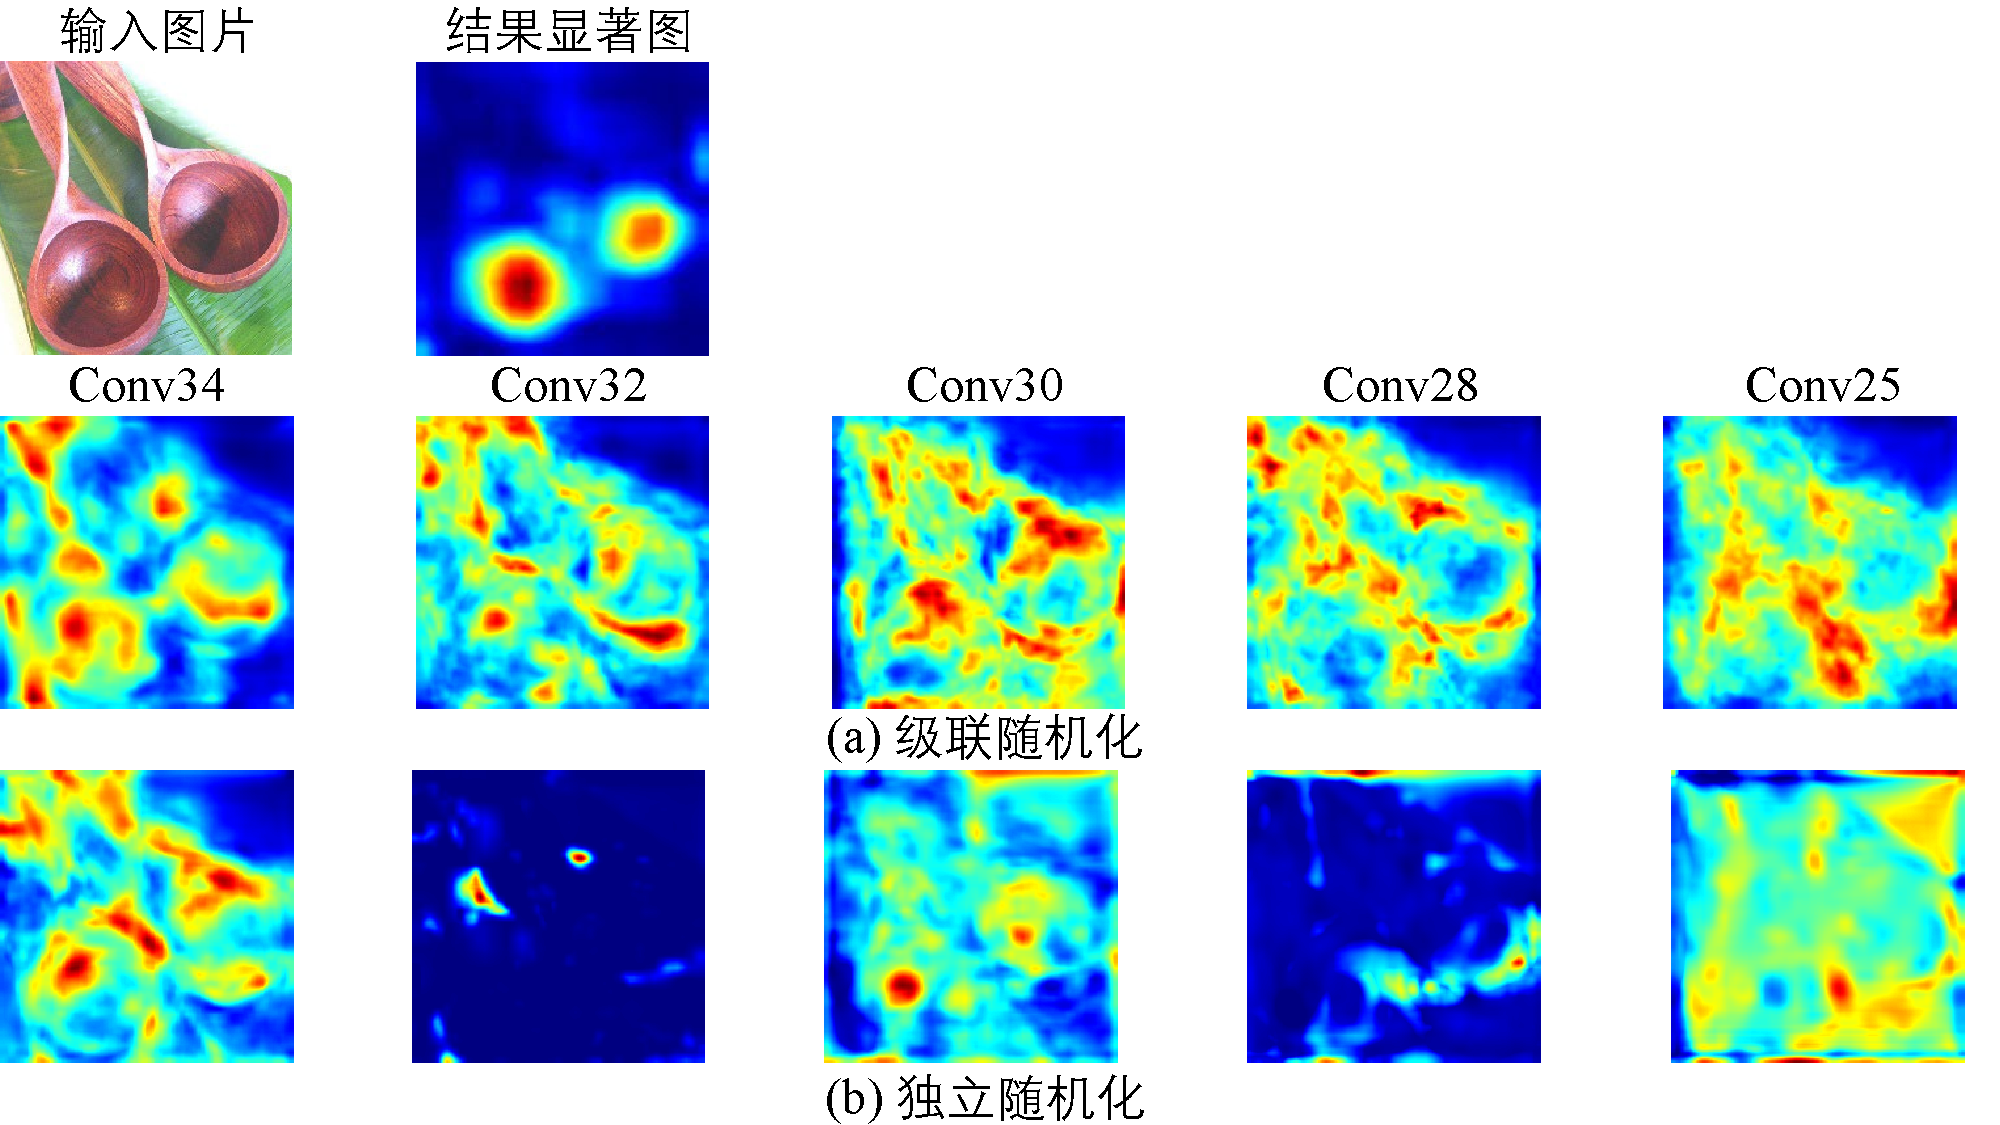
\includegraphics[width=15cm]{fig/ch3/sanityCheck.pdf}
	\bicaption[\xiaosi MSG-CAM合理性检验]{\wuhao MSG-CAM合理性检验示意图}{\wuhao Sanity check of MSG-CAM}
	\label{fig:sanitycheck}
\end{figure}


\section{本章小结}\label{3:finish}
本章首先分析了当前许多针对卷积神经网络的显著图解释方法生成的显著图分辨率的原因,进而引出本章提出的基于输入图片多尺度放大的显著图解释方法,该方法利用卷积核的特性,通过从卷积层提取多个不同分辨率的特征图集合和梯度矩阵,再将它们进行融合作为掩膜来扰动输入图片,从而获得高分辨率和高清晰度的特征图。然后本章设计了插入与删除实验评估该方法生成的显著图中的重要特征区域对图像分类模型给出的预测结果的重要性,之后还设计了定点游戏实验衡量本章方法的显著图的特征定位能力,最后通过直观对比和量化指标对比可以得出本章方法的有效性。